\documentclass[a4paper]{article}

%% Language and font encodings
\usepackage[english]{babel}
\usepackage[utf8x]{inputenc}
\usepackage[T1]{fontenc}

%% Sets page size and margins
\usepackage[a4paper,top=3cm,bottom=2cm,left=3cm,right=3cm,marginparwidth=1.75cm]{geometry}

%% Useful packages
\usepackage{amsmath}
\usepackage{graphicx}
\graphicspath{ {images/} }

\usepackage[colorlinks=true, allcolors=blue]{hyperref}

\title{Assignment 4 - Design an Implementation of your System (DIS)}
\author{ by Group 3 - Plant-Id \\* \\* Team Members: \\* Ethan Ahuja - ahujae \\* Ethan Patterson - patteret \\* James Barry - barryj \\* Evan Brass - brassev \\* \\* Customers: \\* Ethan Ahuja - ahujae \\* Ethan Patterson - patteret}
\begin{document}
\maketitle
\pagebreak
\tableofcontents
\pagebreak
\section{GitHub Link}
As requested in the assignment description, the GitHub branch for this assignment can be found here: \url{https://github.com/barryjosu/CS361-001-W2018/tree/assignment-4}
\section{UML Class Diagram}
\paragraph{Description:}
There will be two systems in our application diagram. One system will handle the client side and the other will handle the server side of our application.
\paragraph{Client side:}
The client system is responsible for interacting with the user. and sending all appropriate data back to the server system.
\paragraph{Server side:}
The server system is responsible for updating the the client system and handling any data the client system pushes.
\begin{center}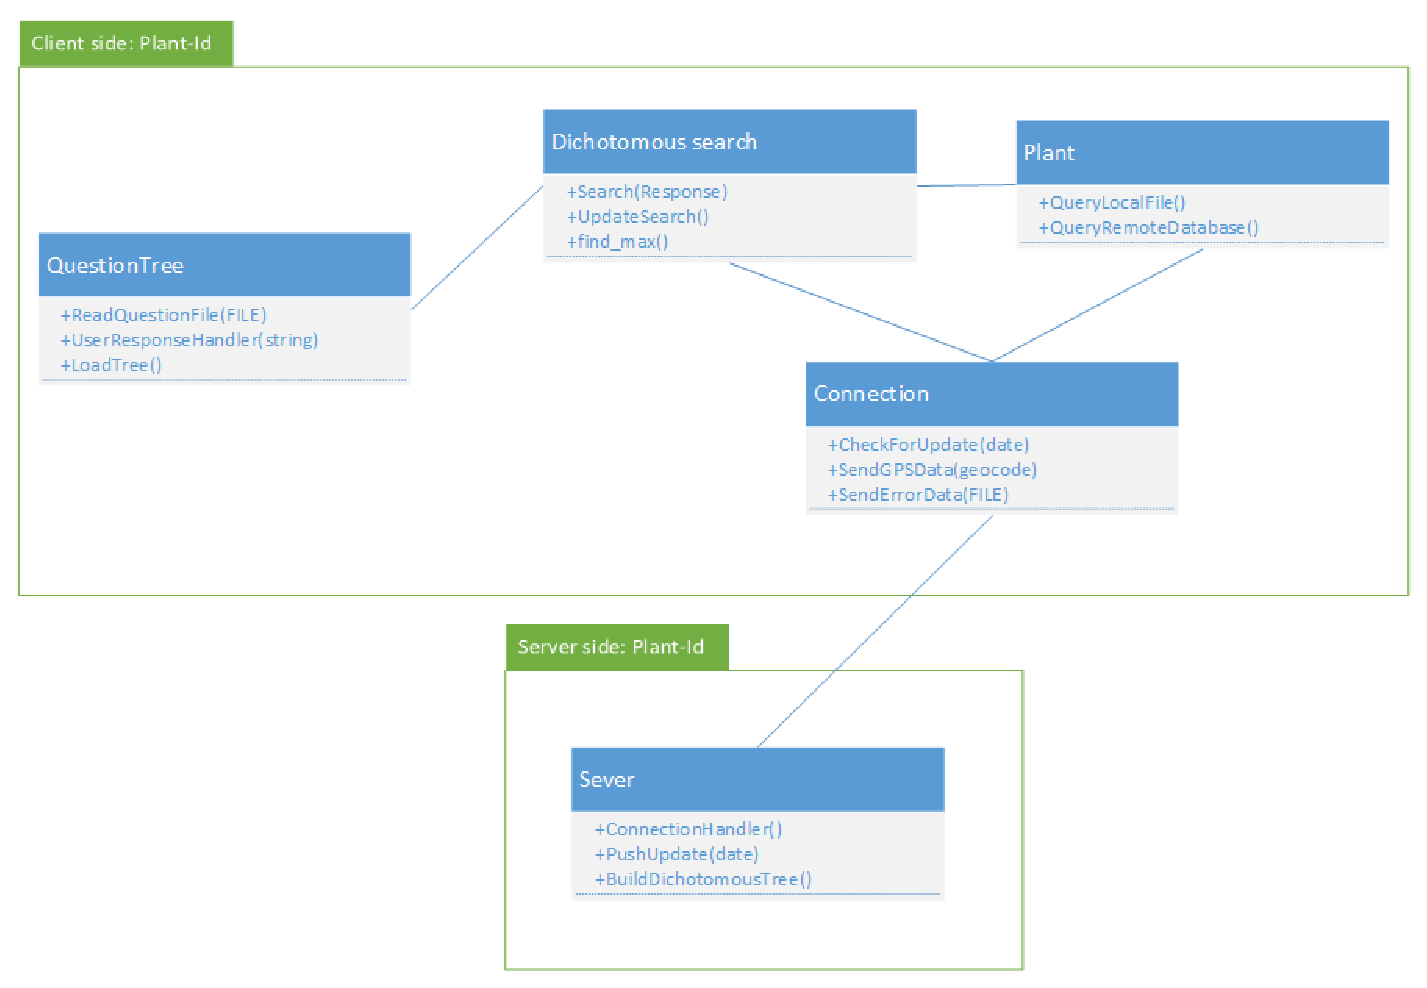
\includegraphics[scale=.7]{UML.eps}\end{center}
\pagebreak
\section{Packages}
Our packaging system is relatively simple. We are using a SQL database to invoke a packaging system by storing key information in different tables. All that the client actually does is query that database. As a result, we will essentially have a client and database package. The client package will handle asking the user questions and using the answers to those questions to query the database. The database is not technically a package, but the sent queries will be handled on the side of the database and the results will be returned to the client. 

The database will be split into three key sections: plants, questions, and reports. The plants section will contain all important information related to our plants, including their name and various features. They may also have an image associated with them, but we are considering instead grabbing images through an automated Google query rather than storing them server- or app-side. We have decided to implement the questions section using a binary decision tree due to the simplicity of implementation, so our questions section will contain all of the "yes" or "no" questions that the user will be asked. The reports section will contain all user feedback and geotag information for plant discoveries. These reports are used to improve the database as well as document locations where particular plants are growing. Using this database will lead to low coupling and high cohesion, as all of our stored data will be fragmented and could be updated independently of other information. However, it will make the app more dependent on an internet connection as the database will always have to be queried. Navigating the stored information would also be very complicated, as we would have to develop associations between different plants in the database in order to navigate through them during the question process.

Below is a SQL table diagram. It explains how our data would be packaged if we chose to implement our information as a database.

\begin{center}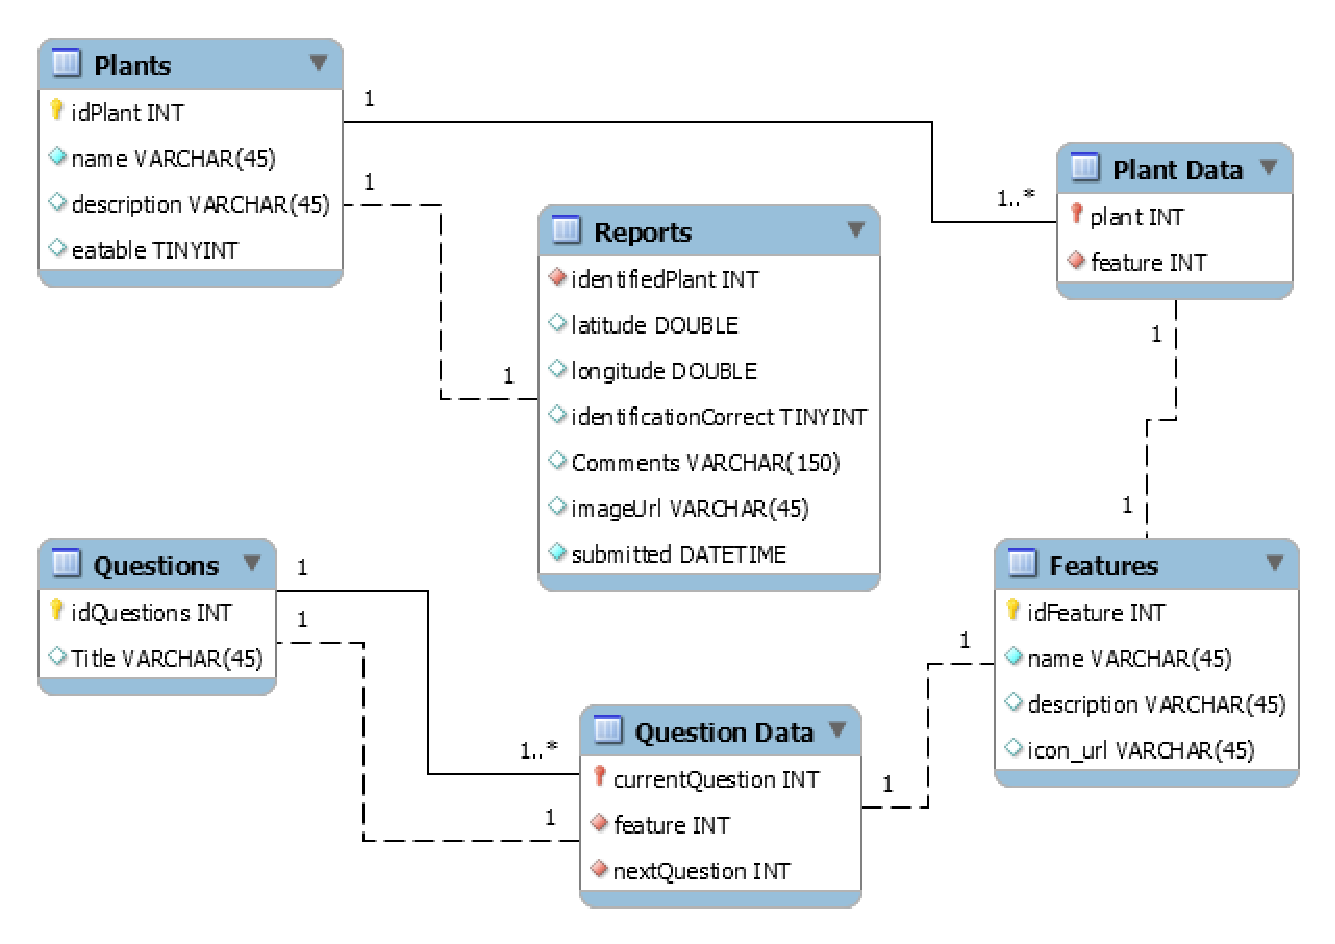
\includegraphics[scale=.6]{DatabaseDesign.eps}\end{center}

In terms of coupling and cohesion, we have tried to separate this package into four parts. The reports section and the Features will remain independent, while the last two sections separate Plants and Questions and their respective data. As new plants are added new questions must follow and that is simply how running a database goes, but it will not affect features or reports as those are general independent parts.

An alternative implementation we are considering is to instead store all of this information in a tree data structure, with each node containing a question and each leaf (node with no branches coming off of it) containing a plant. This would allow us to simplistically navigate down the tree based on the user's answers to questions. This means we would instead have to store a local version of this tree on the user's app and push updates to it when appropriate. it would make our packaging much simpler, but it could lead to higher coupling and lower cohesion, as the user will have to download the entire tree when updates are available in order to ensure accuracy of the tree. It will likely be more simplistic in the grand scheme due to how efficiently the tree could be navigated, though, even without an internet connection. Due to these advantages, we are leaning towards using this implementation.

\pagebreak

\section{Design Patterns}

Through extensive discussion, we have determined that no design patterns particularly benefit our design. Our system is fairly simple. Its goal is to be both basic but helpful, as well as contain a wealth of information. As a result, using a design pattern would unnecessarily complicate our system. A common criticism of design patterns is actually that they lead to inefficient solutions, as a system that's designed well in the first place - or designed so simplistically that it doesn't need any further abstraction - does not benefit from following a pattern \cite{patterns}. 

Despite not following a pattern, we will still be following the principles of object oriented programming. Depending on if we implement with a SQL database or a tree structure (explained in the Packages section), our application will be split into various objects. 

We are leaning towards implementing using a tree structure. If we go with that implementation, we will have...

\begin{itemize}
\item A tree object, which contains pointers to different questions and plants. The "yes" or "no" answer to the questions at each node will determine which node to move to next. If a plant is found rather than a question, then the system knows that the plant in question has been identified. This object will also 
\item Plant objects, which will represent individual plants and contain all of their special properties. These properties include name, edibility, common names, if the plant is dangerous to touch, and possibly more. This information can be grabbed using methods and displayed to the user when the system has identified the plant in question.
\item Question objects, which will contain the question for each node. This will lead to low coupling and high cohesion, allowing us to edit questions without needing to edit the tree, since nodes in the tree will contain pointers to questions. It also allows us to use the same question at multiple points in the tree.
\item A dichotomous search object, which will contain methods related to navigating the tree. This allows us to return information to the user, as well as build the tree when new information is introduced to the database.
\item A server object, which will contain methods for establishing a connection with the user and updating their local version of the tree. It will also allow the user to send feedback to the developers.
\end{itemize}

Due to this inherent simplicity in our objects, a design pattern isn't really needed. All plants have the same set of attributes, so we don't need any sort of polymorphism or inheritance. All our questions simply contain a question, and the tree handles moving between questions. Because of all of the above, we have chosen to not follow any of the design patterns covered in class. 

\pagebreak

\section{Error Handling and Exceptions}

There are various errors we will need to handle in our program. Actual errors are simply connection errors. We will also have logic errors that can be caught by users.

Connection issues will be handled in the typical way. We will implement methods to catch when establishing a connection returns an error. This includes the application connecting to the server for updated, as well as the application connecting to Google to get an image for a plant. We will also handle the case where the user does not have an internet connection, as neither of these features will be available in this case.

Logic errors will be handled using our feedback system. If a user thinks the plant they are trying to identify is not the plant that our tree decides it is, they will be able to report this feedback to the server so that the developers are able to consider it and make changes if needed. We will also have dead ends in our tree, meaning that no plant will be identified based on the answers of the user. This will display a generic message explaining to the user that their plant could not be identified. They will then be given the option to return to the start page for the application.

We are also considering allowing the user to send in images to the developers to help handle these logic errors. If the system fails to identify a plant, it would be helpful to be given an image of the plant the user was trying to identify. This would be a complex system, though, as receiving an image from the user is taxing when compared to receiving text. Getting bad information from the user could also be common, so there would be fake and inaccurate reports to sift through. These issues don't mean the image sending system isn't worth implementing, however, as the reports received that are actually good would be very beneficial to database upkeep. We will look into implementing this once the core features of plant identification have been implemented. 

\pagebreak
\section{Meeting Report}
\textbf{02/10/2018 (2:00pm - 5:00pm):} Johnson Hall - Room 219
\begin{itemize}
\item \textbf{Progress made this week:} James Barry and Ethan Patterson discussed the new, and preferred, choice of implementing a dichotomous search algorithm over the decision tree algorithm. We believe this algorithm will perform more efficiently on the task at hand in comparison to the decision tree.
\item \textbf{Plans and goals for next week:} Goals for next week will be to implement a simple binary tree that uses the dichotomous search algorithm.
\item \textbf{Member contribution:} James Barry and Ethan Patterson met on February 10th from 2 to 5. James compiled sections: Packages, Design Patterns, and Error Handling. Ethan Patterson worked on the UML class diagram. 
\end{itemize}
Meeting Report 2

\textbf{02/12/2018 (4:00-6:00pm):} Valley Library
\begin{itemize}
\item \textbf{Progress made this week:} Ethan Patterson and Ethan Ahuja worked on the presentation and some sections in assignment 4.
\item \textbf{Plans and goals for next week:} Goals for next week will be to the same as the last meeting.
\end{itemize}

\newpage %Move references to the next page..
\begin{thebibliography}{9}
\bibitem{latexcompanion} 
\url{http://www.saedsayad.com/decision_tree.htm}
Dr. Saed Sayad, Reading, www, 2010-2018.
\bibitem{einstein} 
Victor Lavrenko.
\url{https://www.youtube.com/watch?v=eKD5gxPPeY0&list=PLBv09BD7ez_4temBw7vLA19p3tdQH6FYO}
\textit{School of Informatics} 
[\textit{Decision Trees}]. 
Victor Lavrenko and Nigel Goddard, January 19, 2014.
\bibitem{3blueOneBrown}
[\textit{Neural Network}]
YouTube, YouTube, 5 Oct. 2017, \url{www.youtube.com/watch?v=aircAruvnKk&list=PLZHQObOWTQDNU6R1_67000Dx_ZCJB-3pi}
\bibitem{Nielsen, Michael A}
[\textit{Neural Network}
Nielsen, Michael A. “Neural Networks and Deep Learning.” Neural networks and deep learning, Determination Press, 1 Jan. 1970,\url{ neuralnetworksanddeeplearning.com/}.
\bibitem{patterns}
Design Patterns and Criticisms
\url{https://sourcemaking.com/design_patterns}
\end{thebibliography}

\end{document}